\chapter{Felhasználói dokumentáció}
\label{ch:user}

\section{Rendszerkövetelmények}

\begin{itemize}
    \item Hardver
    \begin{itemize}
        \item 2 GHz vagy nagyobb órajelű processzor
        \item 2 GB RAM memória
        \item 1 GB lemezterület a RefactorErl, Visual Studio Code, Erlang LS, illetve a bővítmény számára (forráskódok betöltéséhez további tárhely és memória szükséges)
    \end{itemize}
    \item Szoftver
    \begin{itemize}
        \item mac OS El Capitan, Windows 10 vagy Linux operációs rendszer
        \item Telepített RefactorErl elemző eszköz
        \item GraphViz ??? \todo{Graphviz?}
        \item Erlang/OTP 22 vagy újabb \todo{22?}
        \item Visual Studio Code \todo{Version?}
        \item GCC 4.7.2 vagy újabb fordítóprogram
    \end{itemize}
\end{itemize}

\section{Telepítés}
\subsection{Erlang/OTP telepítése}

Mind a RefactorErl futtatásához, mind az Erlang LS futtatéséhoz szükségünk van az Erlang virtuális gép telepítéséhez. Ezt macOS operációs rendszer legegyszerűbben a Homebrew\footnote{\url{https://formulae.brew.sh/formula/erlang\#default}} nevű csomagkezelővel tehetjük meg. Linux és Windows rendszerekhez az Erlang\footnote{\url{"https://www.erlang.org/downloads"}} honlapjáról tájékozódhatunk a telepítő parancsokról, illetve innen tölthetjük le a telepítő állományt is.

\subsection{RefactorErl telepítése}


\subsubsection{[függőségek telepítése]}
\todo{Függősgek, és YAWS}

A RefactorErl egy nyílt forráskódú szoftver, a forráskód letölthető az eszköz honlapjáról.\footnote{https://plc.inf.elte.hu/erlang/refactorerl-releases.html} Miután kicsomagoltuk az ezközt az alábbi parancs segítségével egyszerűen az alábbi parancs segítségével telepíthetjük:

\lstinline{bin/referl -build tool}

\todo{Referl install}
\todo{brew installer?}

\subsection{Visual Studio Code telepítése}
A Visual Studio Code egy cross-platform\footnote{többféle rendszeren képes futni} fejlesztői környezet, ami igen gazdag fejlesztői interfésszel rendelkezik, ami lehetővé tette ezt a fejlesztést is. Megfelelő operációs rendszer kiválasztása után letölthető a termék honlapjáról. \footnote{\url{https://code.visualstudio.com}}

\subsection{RefactorErl Visualiser telepítése}
A Visualiser bővítmény letölthető a bővítmény GitHub oldaláról \footnote{todo\todo{Git oldal}} vagy a mellekélt állományok között is megtalálható a \lstinline{.vsix} kiterjesztésű telepítő fájl. 


\begin{figure}[H]
  \centering
  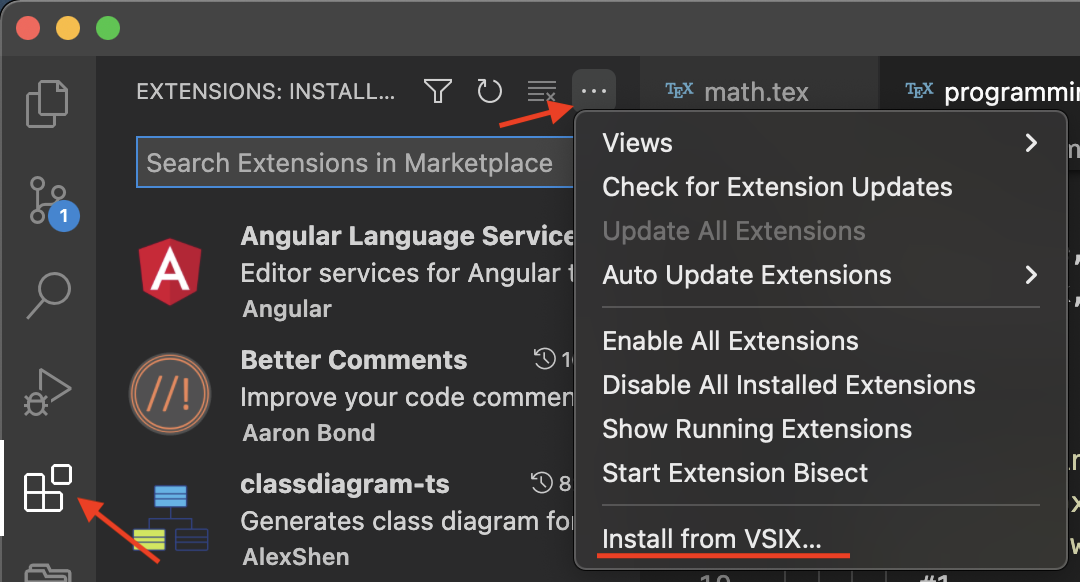
\includegraphics[width=\linewidth]{images/vsix_install.png}
  \caption{Telepítés \lstinline{.vsix} fájlból}
  \label{fig:vsix_install}
\end{figure}

\subsection{Erlang LS bővített változatának telepítése}
Az Erlang Language Server \textit{eredeti verziója} megtekinthetó a GitHub tárolójában \footnote{todo\todo{LINK A GITHUBHOZ}}, illetve letölthető a Visual Studio Code Marketplace\footnote{todo\todo{LINK AZ ERLANG LS}}-ről 




\section{Erlang LS használata}
\subsection{Első elindításkor szükséges beállítási lehetőségek} \label{ELSfirstStart}
Az első elidulás előtt az Erlang LS konfigurációs fájljában néhány módosítást kell végeznünk, hogy az megfelelően illeszkedjen a RefactorErlhez. A konfigurációs fájl YAML formátumot követ. 
A diagnosztikák futtatásához vegyük fel a \lstinline{refactorerl} elemet az engedélyezettek közé. 

\lstset{caption={RefactorErl diagnosztikák engedélyezése Erlang LS-ben}, label=src:yaml}
\begin{lstlisting}
diagnostics:
  enabled:
    - refactorerl
\end{lstlisting}

Ezzel a beállítással az Erlang LS már futtatni fogja a diagnosztikákat, azonban alapértelmezetten egyetlen diagnosztikai sem fog futni, ezeket manuális allíthatjuk be. Ehhez vegyünk fel egy \lstinline{refactorerl} kulcsot a fájl gyökerébe. Ez alá két \textit{alkulcs} kerülhet:
\begin{itemize}
    \item \lstinline{node}: ide annak az Erlang node\todo{Errre mi a magyar terminológia?}-nak a nevét kell megadni szöveges karakterláncként, ahol a RefactorErl fut. 
    \item \lstinline{diagnostics}: azon diagnosztikák azonosítói, amelyeket futtatni szeretnék listként (felsoroláskén) megadva. A dignosztikák azonosítói szintén szöveges karakterláncok.
\end{itemize}

Példa egy ilyen konfigurációs fájl részletre:

\lstset{caption={RefactorErl konfigurációs példa Erlang LS-ben}, label=src:yaml}
\begin{lstlisting}
diagnostics:
  enabled:
    ...
    - refactorerl

...

refactorerl:
  node: "nodeName@hostName" 		
  diagnostics:
    - "unused_macros"			
    - "unsecure_os_call"
\end{lstlisting}

Az alábbi diagnosztikákból tudunk válogatni jelenleg:


\begin{longtable}{|m{0.4\textwidth}|m{0.5\textwidth}|}
 \hline
 Lekérdezés neve & Lekérdezés rövid ismertetése \\ [0.5ex] 
 \hline\hline
 \verb|unused_macro| & Nem használt makró definíciók megjelenítése \\ \hline
 \verb|unsecure_calls| & Az összes lehetséges támadási forma megjelenítése \\ \hline
 \verb|unsecure_interoperability| & Az együttműködési képességből fakadó sebezhetőségek azonosítása. \\ \hline
 \verb|unsecure_concurrency| & A konkurens programozásból eredő hibalehetőségek feltérképezése. \\ \hline
 \verb|unsecure_os_call| & Az ismeretlen helyről származó paraméterekkel meghívott OS szintű utasítások ellenőrzése. \\ \hline
 \verb|unsecure_port_creation| & A portok létrehozásával kapcsolatos sebezhetőségek megjelenítése. \\ \hline
 \verb|unsecure_file_operation| & Az ismeretlen bemenettel meghívott fájlkezeléssel kapcsolatos műveletek megjelenítése. \\ \hline
 \verb|unstable_call| & Az atomok dinamikus létrehozásával kapcsolatos függvények feltérképezése. \\ \hline
 \verb|nif_calls| & A NIF függvények használatából fakadó sebezhetőségek ellenőrzése. \\ \hline
 \verb|unsecure_port_drivers| & A dinamikusan betölthető könyvtárak használatából fakadó veszélyek azonosítása. \\ \hline
 \verb|decommissioned_crypto| & Az elavultnak számító kriptográfiai műveletek megjelenítése. \\ \hline
 \verb|unsecure_compile_operations| & Az ismeretlen helyről származó programkód fordításának és betöltésének ellenőrzése. \\ \hline
 \verb|unsecure_process_linkage| & A folyamatok nem megfelelő összekapcsolásából adódó sebezhetőségek megjelenítése. \\ \hline
 \verb|unsecure_prioritization| & A folyamatok prioritásának módosításából fakadó veszélyek ellenőrzése. \\ \hline
 \verb|unsecure_ets_traversal| & Az ETS tábla rögzítés nélküli bejárásának ellenőrzésére szolgáló megjelenítése. \\ \hline
 \verb|unsafe_network| & A hálózati rendszermaggal kapcsolatos műveletek feltérképezése. \\ \hline
 \verb|unsecure_xml_usage| & Az ismeretlen helyről származó xml paraméterek elemzésével kapcsolatos függvények azonosítása. \\ \hline
 \verb|unsecure_communication| & Az elosztott hálózat szereplői között zajló kommunikációs beállítások ellenőrzése. \\ [1ex] 
 \hline
\caption{Elérhető diagnosztikai azonosítók listája.}
\label{table:1}
\end{longtable}



\subsection{Diagnosztikák használata}
Az Erlang LS a diagnosztikákat az adott szerkesztőben figyelmeztetésként jeleníti meg. Ugyan ez a funckionalitás \textbf{minden ELS-el kompatibilis szerkesztőben meg fog jelenni}, most a példák során a Visual Studio Code szerkesztőre fogunk fókuszálni. Miután a konforgurációs fájlban mindent beállítotunk (ld. \ref{ELSfirst} bekezdés) nincs más dolgunk, mint betölteni egy forráskódot és megtekinteni az eredményt.

\subsubsection{Példa: Nem használt makró definíciók}

Az alábbiakban a \lstinline{unused_macros} azonisítójú diagnosztikát fogjuk áttekinteni. Ehhez nézzük meg alábbi a forrást:

\lstset{caption={Nem használt makró definíciókkal eláttot szemléltető kód}, label=src:erlang}
\begin{lstlisting}[language={Erlang}]
-module(show).
-define(PRIME, 7).
-define(NOT_PRIME, 12).

show_prime() ->
    ?PRIME.
\end{lstlisting}

Itt láthatjuk, hogy a \lstinline{NOT_PRIME} makró az nincsen használatban. Ha megnézzük, milyen diagnosztikákat kaptunk a RefactorErl-től, az Erlang LS-en keresztül akkor láthatjuk, hogy figyelmesztetés szintű diagnosztikát jelez nekünk.

\begin{figure}[H]
  \centering
  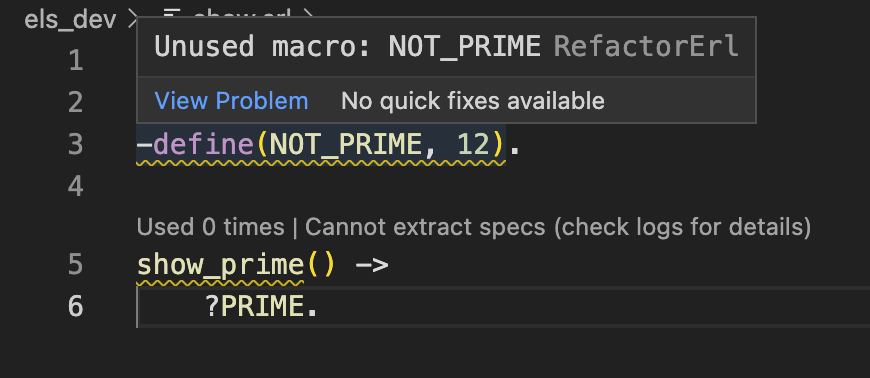
\includegraphics[width=0.7\linewidth]{images/undefined_macro.png}
  \caption{Nem használt makró diagnosztika Visual Studio Code-ban}
  \label{fig:unused_macro_vscode}
\end{figure}


\subsubsection{Példa: Nem biztonságos \lstinline{os} hívás diagnosztika}

\lstset{caption={Nem biztonságos \lstinline{os} hívást szemléltető kód}, label=src:erlang} 
\begin{lstlisting}[language={Erlang}] 
-module(show).
-export([safe_os_call/0, unsafe_os_call/1]).

safe_os_call() ->
    os:cmd("ls").

unsafe_os_call(A) ->
    os:cmd(A).
\end{lstlisting}

A fenti forrásban ötödik sorban lévő \lstinline{os:cmd} hívást nem tekintjük veszélyforrásnak, hiszen a fejlesztő maga paraméterezi fel. Azonban hetedik sorban kezdődő \lstinline{unsafe_os_call} definíciót sérülékenységi pontnak tekintjük, hiszen paramétere ismeretlen helyről származik \cite{refactorerlSecurity} 

Ennek megfelőle a \ref{fig:unsafe_os_call_vscode} ábrán láthatjuk is, hogy a szerkesztő program figyelmeztetést is adott a szóbanforgó kódrészletre. 

\begin{figure}[H]
  \centering
  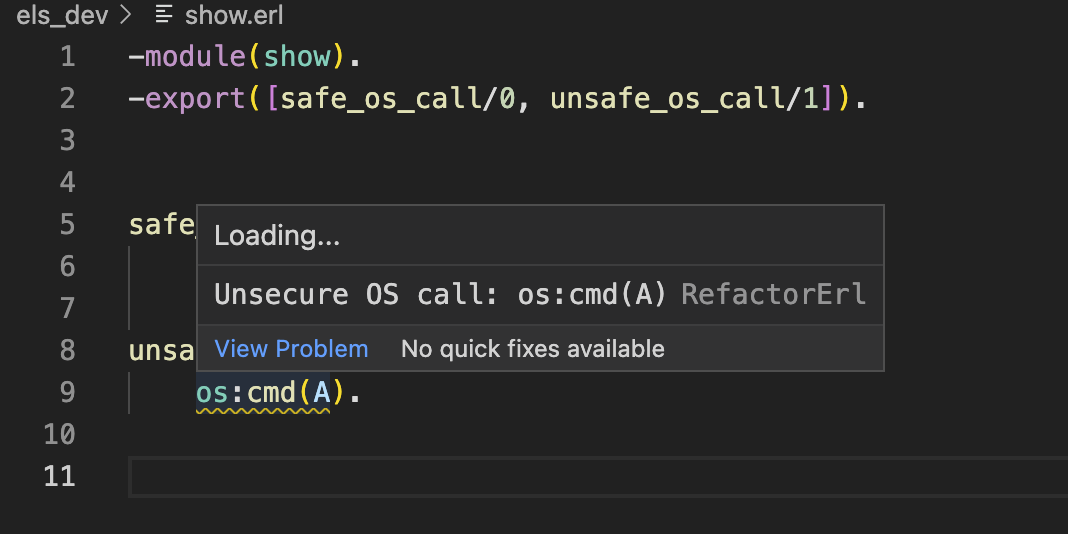
\includegraphics[width=0.7\linewidth]{images/unsafe_os.png}
  \caption{Nem biztonságos \lstinline{os} hívás diagnosztika Visual Studio Code-ban}
  \label{fig:unsafe_os_call_vscode}
\end{figure}

Ezen fejezetnek nem célja bemutatni az összes lehetséges diagnosztikát, csupán egy átfogó képet adni, azok használatáról. Továbbiakban az felhasználóra van bízva, hogy mely diagnosztikát szeretné használni. Az integrált diagnosztikák jelentős része Baranyai Brigitta TDK dolgozatából származik, ahol további részletekről is olvashatunk. \cite{refactorerlSecurity}


\subsection{Kódakció parancsok kiadása}
A kódakciók, avagy angolul \textit{Code Actions} a fejlesztői környezetben megjelenő gyors javítások, refaktorálások és tanácsok. Jelenleg inkább az első kettő megközelítés az elterjedt, ahogyan azt a Visual Stuido Code felhasználói útmutatója is írja. \cite{vscodeCodeActionUserGuide} Ebben a dolgozatban ezen funkciót kissé kiterjesztve, kód értelmezési funkcionalitást kapott. Kódakcióként elérhetőek az alábbi funkciók:

\begin{itemize}
    \item Függőségi gráf lekérése adott függvény... \todo{fv? gráf?} fv hívás modul
    \item Változó \todo{origin??} origonjának lekérdezése
    \item Változó \todo{reach} reachjének lekérdezése
\end{itemize}

Ugyan a fent felsorolt funkcionalitások az Erlang LS felületéről indulnak, azonban sajnos a \textit{Language Server Protocol} limitációi miatt, ezen funkciók, lekérdezések megjelenítésére nincsen lehetőség. \cite{microsoftLSp} Ezen limitációk áthidalására készült a RefactorErl Visualiser bővítmény.

\todo{hivatkozás arra, hogy ez miképpen fog megjelenni}

\section{Visualiser kiegészítő használata}
\subsection{Elindítása}

Az elindításhoz nincsen más teendőnk, mint az oldalsávon megjelenő RefactorErl logóra kattintani. 

\begin{figure}[H]
  \centering
  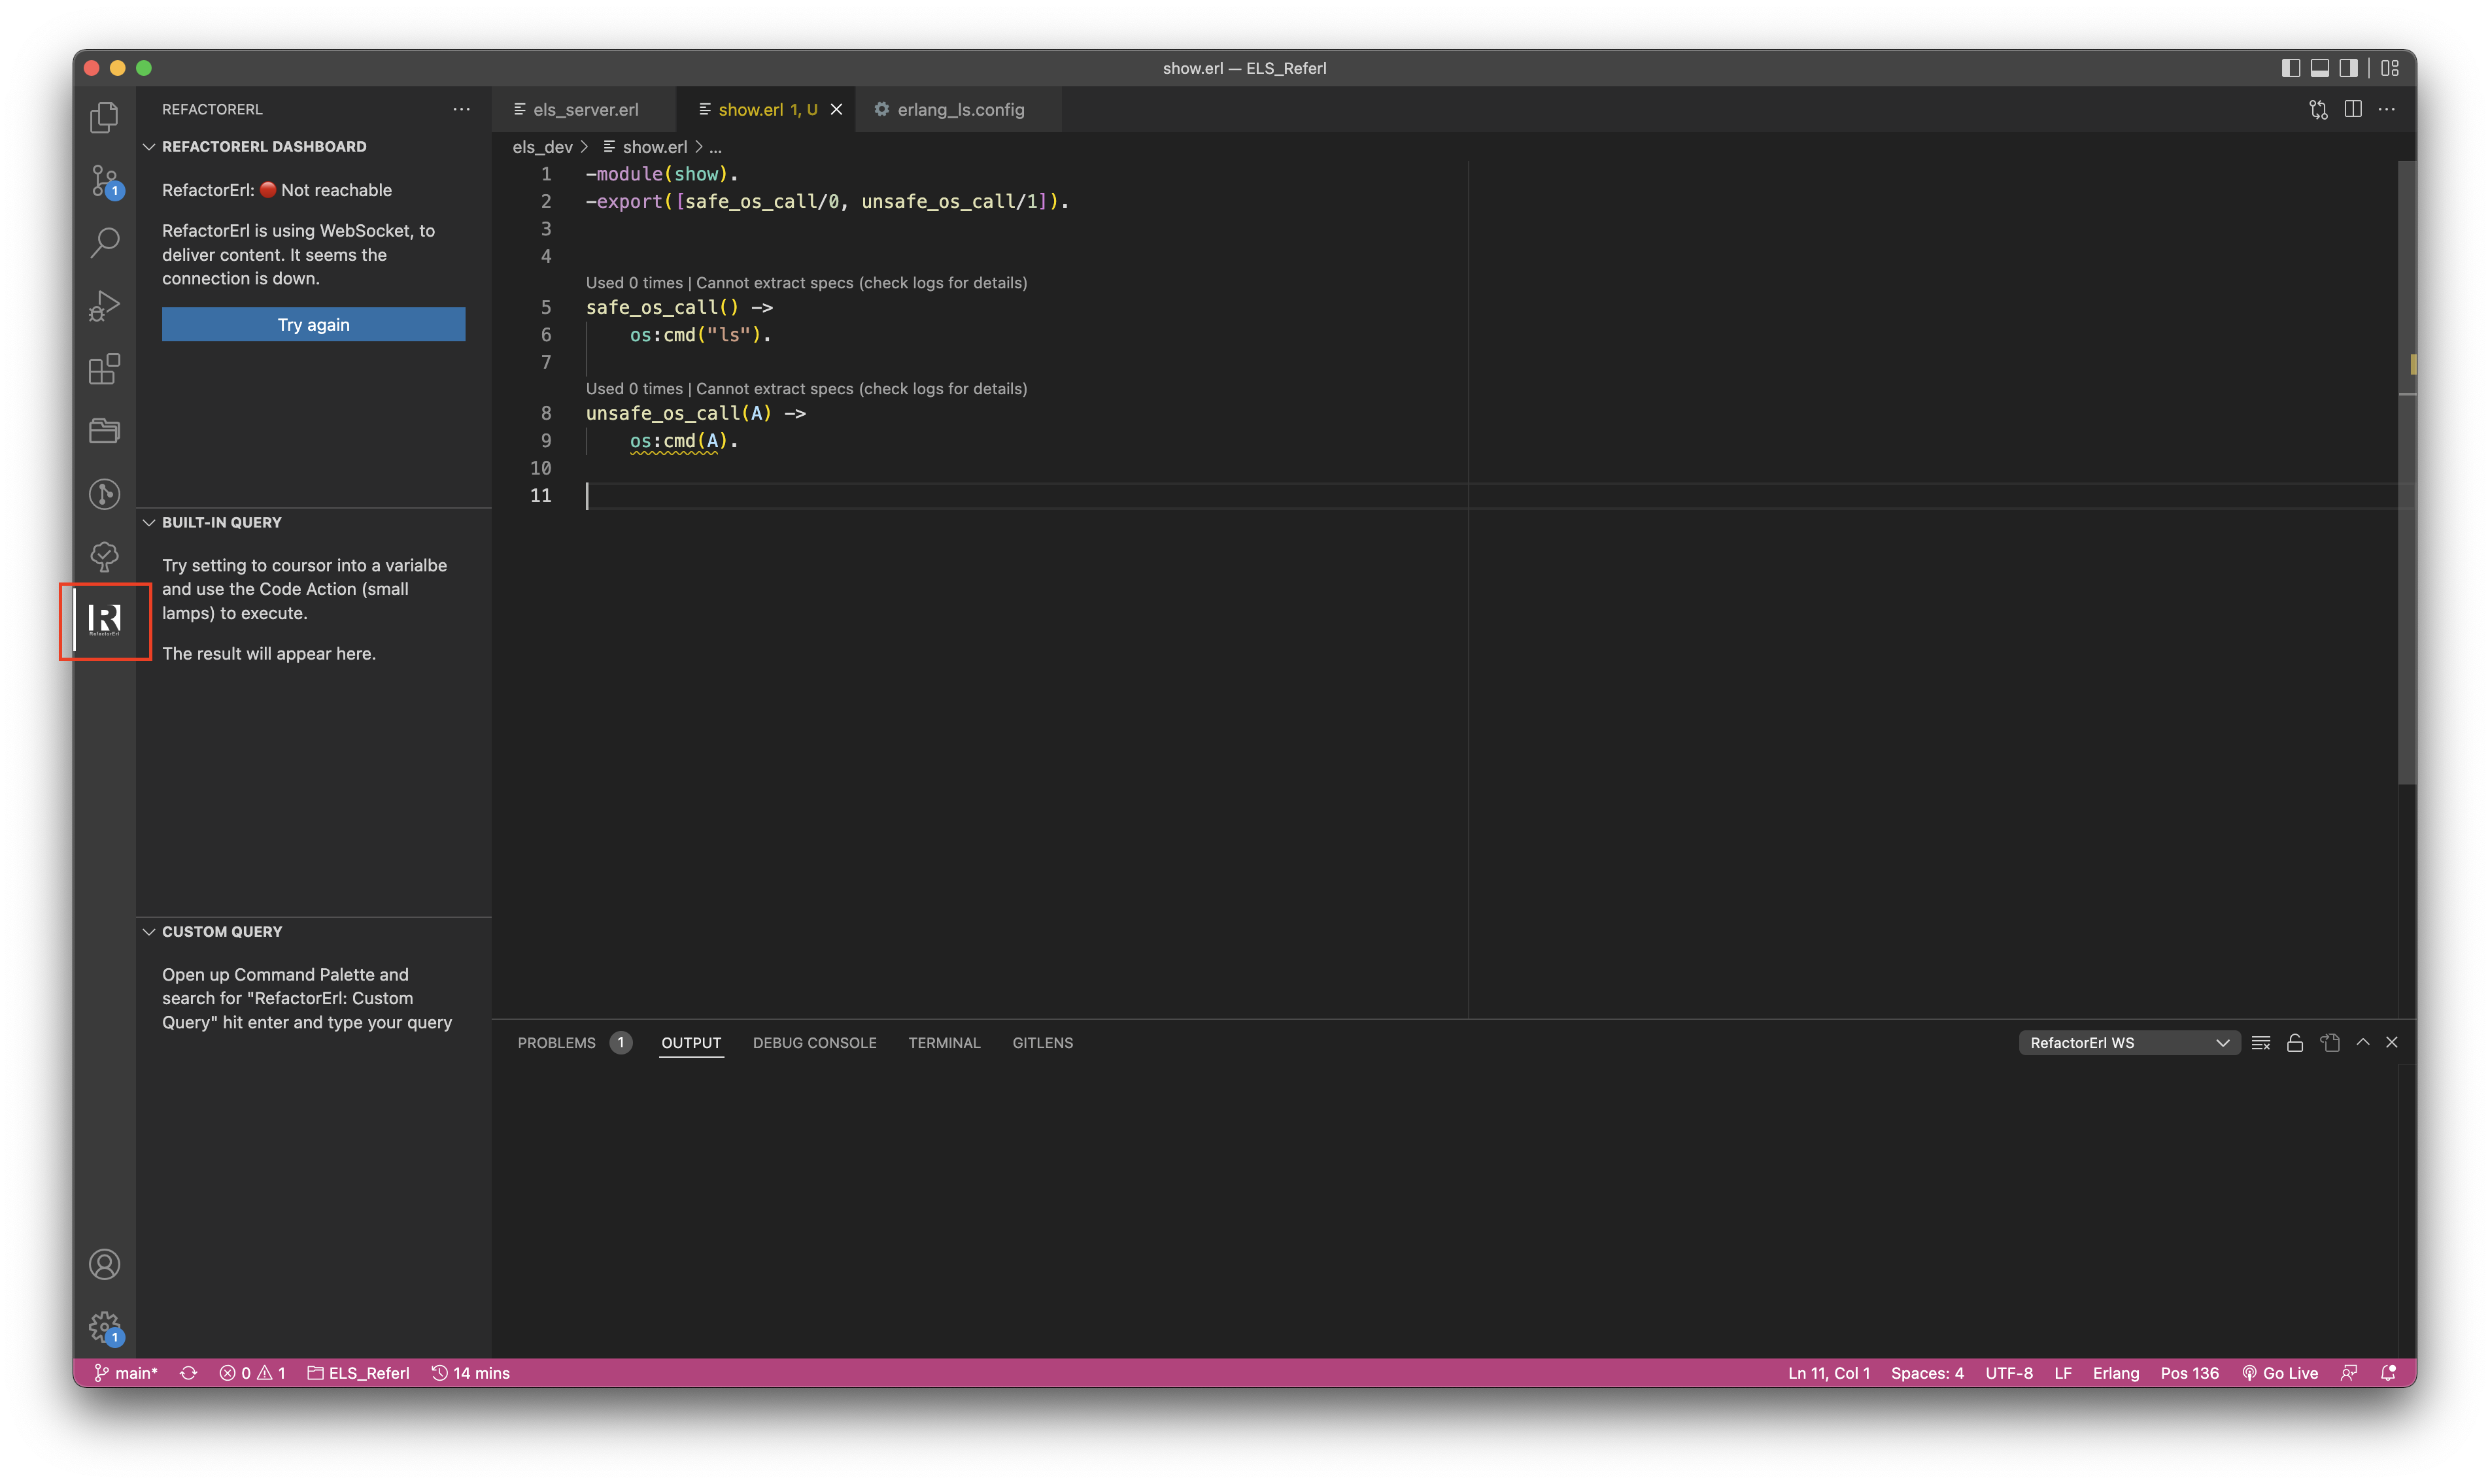
\includegraphics[width=\linewidth, clip=true, trim = 0mm 0mm 150mm 0mm]{images/start_visualiser.png}
  \caption{RefactorErl Visualiser indítása}
  \label{fig:start_visualiser}
\end{figure}

\todo{szemléltetés, screenshot} szemléltetés, screenshot

\subsection{Egyéni szemantikus lekérdezések}
A kiegészítő segítségével egyedi szemantikus lekérdezéseket is futtathatunk a RefactorErl adatbázisában tárolt fájlokon. A szemantikus lekérdezéseket az eszköz lekérdező nyelvének segítségével foglmazhatjuk meg, melyről bővebb információt a projekt wiki oldalán találhatunk \todo{cite!!}

Ahhoz, hogy egy ilyen lekérdezést futtassunk az ún. \textit{Command Pallette}-et nyissuk meg, amit mac OS-en a \lstinline{CMD + SHIFT + P}, Windows-on és Linux operációs rendszeren pedig a \lstinline{CTRL + SHIFT + P} billenytűk egyidejű lenyomásával tudunk elő hozni. Itt kezdjük el gépelni a parancs nevét: \textit{Custom Query}, majd a megjelenő lehetőségek közül válasszuk ki a \textit{RefactorErl} prefixxel ellátott opciót.

\begin{figure}[H]
  \centering
  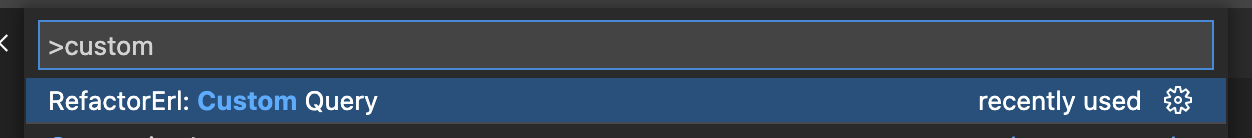
\includegraphics[width=\linewidth]{images/custom_query_palette.png}
  \caption{Custom Query megnyitása a Command Palette felületéről}
  \label{fig:custom_query_palette}
\end{figure}

Ez után a \textit{Command Palette} helyén megjelenik egy beviteli mező, ahova beírhatjuk a lekérdezést.

\begin{figure}[H]
  \centering
  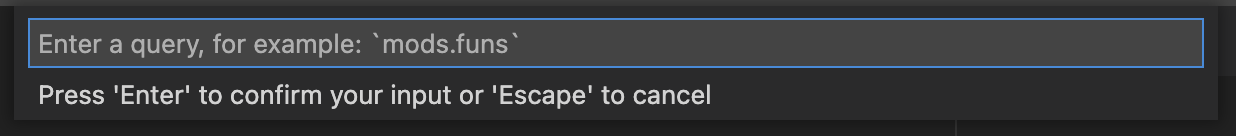
\includegraphics[width=\linewidth]{images/custom_query_input.png}
  \caption{Beviteli mező a Query számára}
  \label{fig:custom_query_palette}
\end{figure}

A lekérdezést az \textit{Esc} billenytű lenyomásával megszakíthatjuk, azt \textit{Enter} segítségével pedig elküldhetjük azt. A lekérdezés állapotáról a jobb alsó sarokban kaphatunk információt.

\begin{figure}[H]
  \centering
  
\includegraphics[width=0.4\linewidth]{images/notification_done.png}
  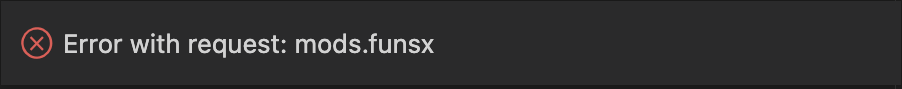
\includegraphics[width=0.4\linewidth]{images/notification_error.png}
  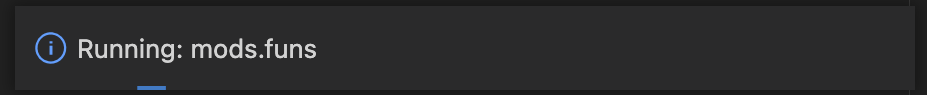
\includegraphics[width=0.4\linewidth]{images/notification_running.png}

  \caption{Lehetséges  értesítések lekérdezés esetén}
  \label{fig:notifications}
\end{figure}

A \ref{fig:notifications} ábrán látottakon túl, időtúllépés miatt is kaphatunk hibát, ez esetben a rendszer egy \textit{TIMEOUT} értesítést küld.



\subsection{Függőségi gráf rajzolása}
\subsection{Változóhoz kapcsolodó lekérdezések megjelenítése}


\subsection{Dinamikus függvény hívások megjelenítése}
\subsection{Kapcsolat ellenőrzése}
\subsection{Adatbázis szinkronizáció elvégzése}
\subsection{Dinamikus hívás elemzés kezelése}
